\documentclass[12pt]{elsarticle}
\usepackage{times}
\usepackage[margin=1in]{geometry}
\pagestyle{empty}
\usepackage{natbib}
\bibliographystyle{unsrt}
\usepackage{color}
\usepackage{amsmath}
\usepackage{hyperref}
\usepackage{wrapfig}
\usepackage{titlesec}
\titleformat{\section}[runin]{\normalfont\bfseries}{\thesection.}{3pt}{}


\begin{document}

\begin{center} \textbf{PROJECT NARRATIVE} \end{center}

%
\section{Goals and objectives} [note the RFP does not require a section for goals and objectives, but I believe a summary upfront will increase readability of the proposal]
\subsection{Goals}
\begin{enumerate}
\item
\item
\item
\end{enumerate}

\subsection{Objectives}
\begin{enumerate}
\item Synthesize methods and datasets for fish passage prioritization for all counties within the Washington state injunction area.
\item Generate a geospatial dataset of current usual and accustomed fishing areas for tribal nations in Western Washington.
\item Generate predicted cost estimates for all barriers to fish passage within the Washington state injunction area. 
\end{enumerate}

%
\section{Background}
\subsection{Fish passage in Washington state}
\subsection{Optimization tools in fish passage}
\subsection{Optimization for Washington fish passage}

%
\section{Approach}
\subsection{Cost model}
\subsection{Habitat model}
\subsection{Equity}
\subsection{Risk mitigation}

\subsection{Network configuration}
\subsection{Ownership}
\subsection{Optimization}

We will explore two alternative approaches to define cost-effective restoration plans that meet multiple planning goals (e.g.\ salmon habitat gains, equity considerations, and risk mitigation). Both approaches are considered ``a priori'' methods for multiobjective optimization because the decision maker must specify their preferences related to the various objectives prior to the optimization. 

\begin{wrapfigure}{R}{0.5\textwidth}
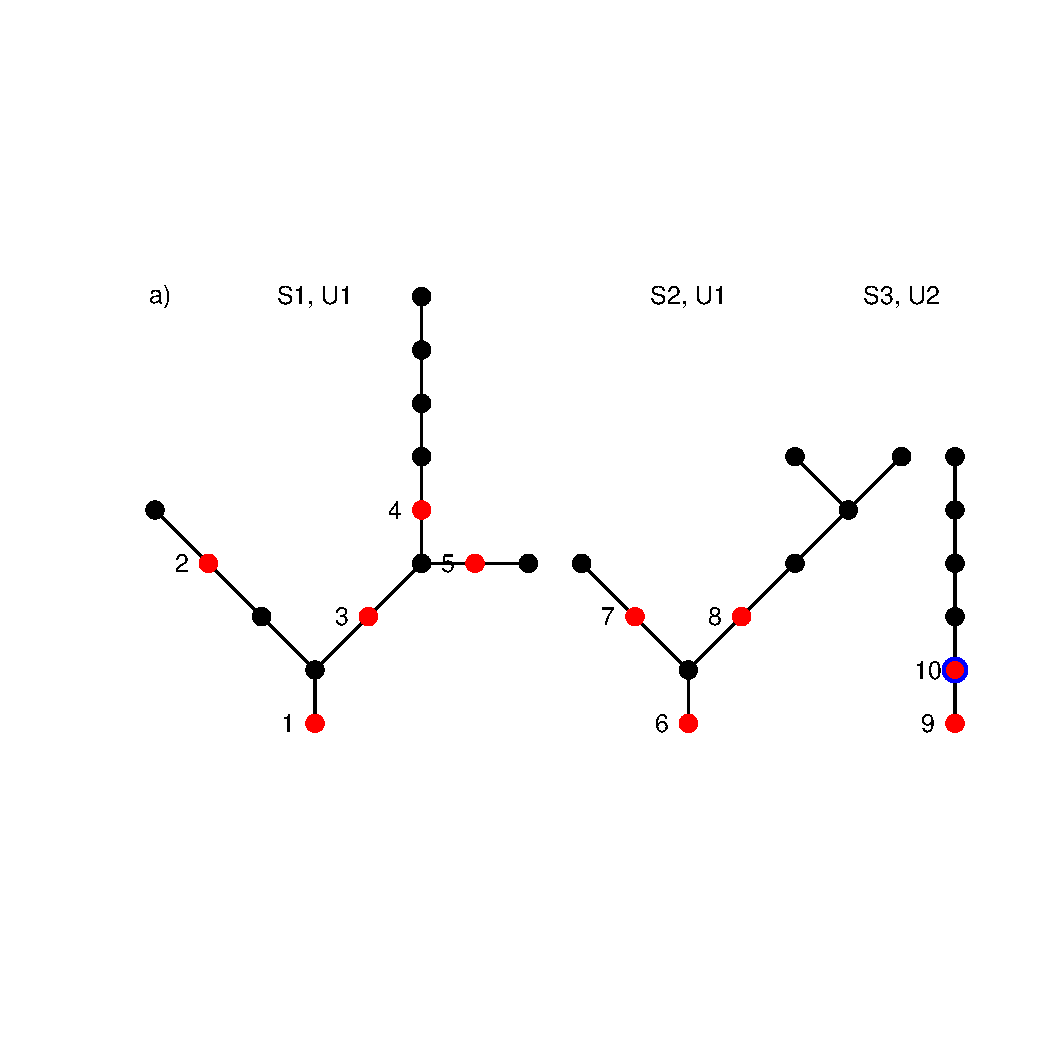
\includegraphics[width=0.48\textwidth]{figures/opt_s.pdf}
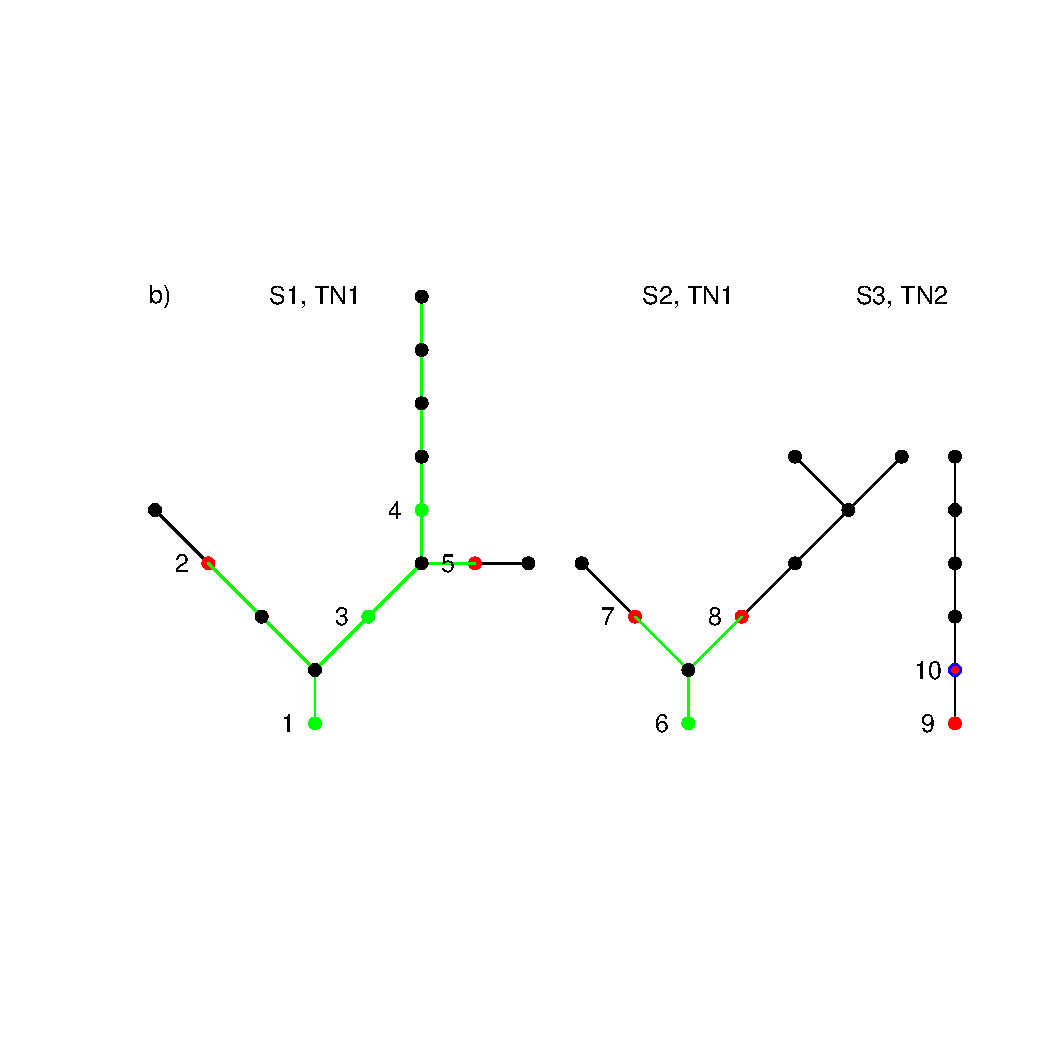
\includegraphics[width=0.48\textwidth]{figures/opt_h.pdf}
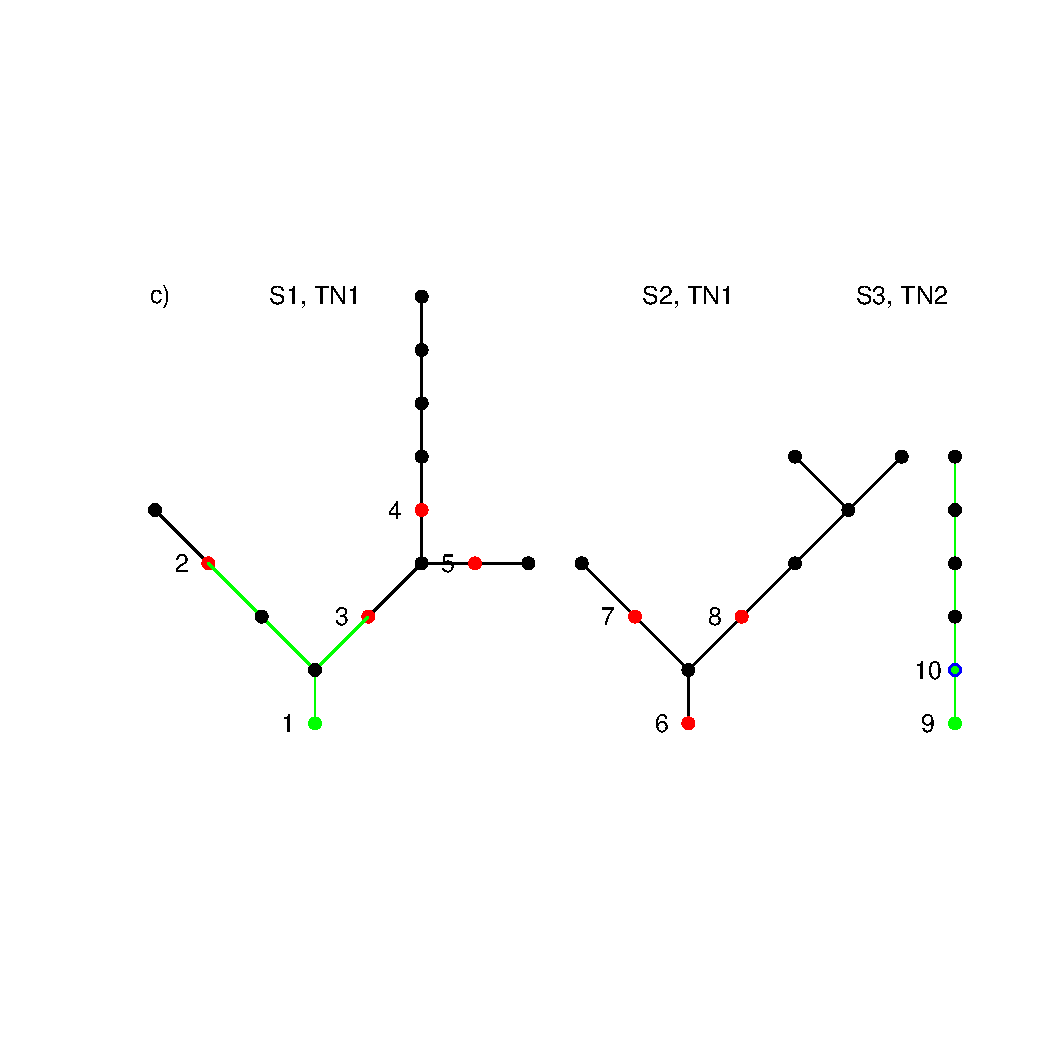
\includegraphics[width=0.48\textwidth]{figures/opt_e.pdf}
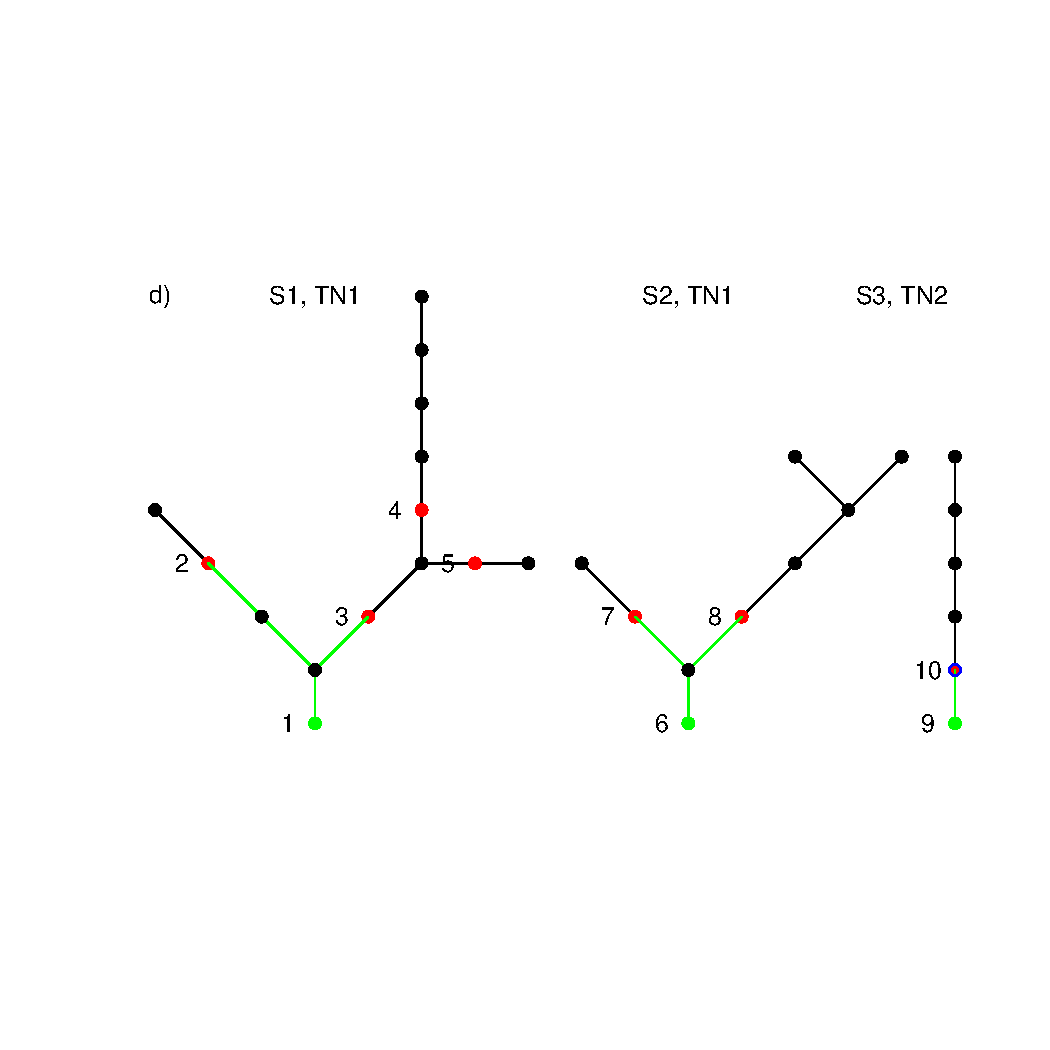
\includegraphics[width=0.48\textwidth]{figures/opt_d.pdf} 
\caption{Solutions to a scalarized multiobjective problem in a stylized system where there are 3 salmon stocks (S1-S3) and 2 tribal nations (TN1-TN2). \label{fig:opt}}
\end{wrapfigure}

In the first approach (i.e.\ linear scalarization), managers specify importance weights for each of the objectives and the weighted sum of the objectives is maximized. Weights are constrained to the interval [0, 1] and sum to one, e.g.\ a manager solely interested in habitat would set the habitat importance weight to 1 and all other weights to zero. The problem will also include a budget constraint, such that expenditures on barrier restoration are less than or equal to a fixed budget $B$, and a hydrography constraint such that habitat gains from restoring any one barrier cannot be realized if there exist any downstream barriers to fish passage. Figure~\ref{fig:opt} demonstrates solutions to this first optimization approach with a budget constraint of \$40. Panel (a) represents a model system with 10 barrier culverts (numbered red markers), 26 units of potential habitat (increments between two adjacent markers represent 1 unit of habitat), on 3 streams utilized by 3 salmon stocks (S1-S3), harvested by two tribal nations (TN1-2). Each of the culverts 1-9 costs \$10 to restore while culvert 10 costs \$20 to restore (and is outlined in blue).

Panel (b) represents the habitat-maximizing solution (the habitat weight is set to one and all other weights are set to zero) , with 14 units of habitat gained (11 on stream 1 and 3 on stream 2), but all of the benefits going to a single tribal nation. In the habitat-maximizing solution, the budget is exhausted by restoring 4 culverts for a total cost of \$40. Panel (c) represents the equity-maximizing approach (the equity weight is set to one and all other weights are set to zero), with 9 units of habitat restored (4 on stream 1 and 5 on stream 3). In this solution, the budget is also exhausted and the habitat gains are nearly evenly split across tribal nations (4 for Tribal Nation 1 and 5 for Tribal Nation 2). Finally, panel (d) represents the diversification-maximizing solution (the weight on diversifying habitat gains across salmon stocks is set to one and all other weights are set to zero), with a total of 8 units of habitat gained (4 on stream 1, 3 on stream 2, and 1 on stream 3) spread across the three salmon stocks. Interestingly, the budget is not exhausted in the diversification-maximizing solution as total expenditures for the 3 culverts restored is \$30. Whenever objective functions are defined by even allocations, e.g.\ across tribal nations or salmon stocks, the budget constraint may not hold.

In the second approach (i.e.\ $\epsilon-$constraint method), one objective function is maximized and lower bounds, $\epsilon$ parameters are provided for all remaining objectives. For example, the problem can be defined to maximize habitat gains subject to each tribal nation receiving some minimum fraction of the habitat gains or some minimum fraction of total expenditures, or a constraint such that habitat gains are distributed across some minimum number of salmon stocks.



%As an illustrative example of the first approach, suppose Lewis County wants to define a restoration plan (a package of culverts to be restored) that balances habitat increases for Chinook salmon in the injunction area with equity and risk mitigation. Further suppose Lewis County had a budget of B dollars to invest in the restoration plan and does not want to restore any culverts outside of its jurisdiction. Our framework would solve the following problem (blue text represents manager inputs):
%\begin{equation*}
%\substack{\text{\large max}}_{\boldsymbol{c}}\hspace{0.25in} \textcolor{blue}{w_1}\:\: \text{Chinook habitat metric} + \textcolor{blue}{w_2}\:\: \text{equity metric} + \textcolor{blue}{w_3}\:\: \text{risk mitigation metric},
%\end{equation*}
%\noindent subject to:  
%\begin{equation*}
%\text{total cost} \le \textcolor{blue}{B} 
%\end{equation*}
%\begin{equation*}
%\boldsymbol{c} \in \{\textcolor{blue}{\boldsymbol{c}_{lewis}}  \},
%\end{equation*}
%\begin{equation*}
%\text{hydrography}
%\end{equation*}
%
%where $\boldsymbol{c}$ are culverts included in the restoration plan, $\boldsymbol{c}_{lewis}$ are the subset of barrier culverts owned by Lewis county, B is total amount of funding that can be spent, and $w_1-w_3$ are the weights that managers place on each objective. The problem will be additionally constrained so that benefits from upstream culvert removal cannot be captured without first removing downstream blockages.
%
%As an illustrative example of the second approach, suppose Lewis County wants to define a restoration plan that maximizes habitat but 



\subsection{Role of team members and partners}
\textbf{PI Jardine} will serve as the lead administrator of the grant where administrative responsibilities include organizing meetings both internally and with the scientific advisory board to ensure the project is on track to deliver work products on time, tracking project performance, facilitating project design decisions, and supervising and mentoring the postdoctoral scholar and the Sea Grant Fellow.  PI Jardine will also provide technical assistance with optimization in R and developing the R Shiny app including providing template code for various optimization algorithms along with sensitivity analyses and model selection, and providing template code for the DST user app features.\\


%
\section{Engagement plan}
\subsection{Community collaborators} 
\subsection{Target audiences}
\subsection{Engagement activities}
\subsection{Anticipated outcomes and evaluation}

\clearpage
\large References\\
\normalsize
\bibliography{wsg}
\end{document}